\documentclass[aspectratio=43]{beamer}
\usepackage[english]{babel}
\usepackage{amsthm}
\usepackage{mathtools}
\usepackage{physics}
\usepackage{calligra}
\usepackage{csquotes}
\usepackage{tensor}
\usepackage[thicklines]{cancel}
\usepackage{tcolorbox}
\usepackage{pstricks}
\usepackage{setspace}
\usepackage[backend=biber, bibstyle=nature, sorting=nty, citestyle=numeric-comp]{biblatex} %Custom bibliography
    \addbibresource{bib.bib} %Load references


\DeclareMathAlphabet{\mathcalligra}{T1}{calligra}{m}{n}
\DeclareFontShape{T1}{calligra}{m}{n}{<->s*[2.2]callig15}{}
\newcommand{\scriptr}{\mathcalligra{r}\,}
\newcommand{\boldscriptr}{\pmb{\mathcalligra{r}}\,}
\def\rc{\scriptr}
\def\brc{\boldscriptr}
\def\hrc{\hat\brc}
\newcommand{\ie}{\emph{i.e.}} %id est
\newcommand{\eg}{\emph{e.g.}} %exempli gratia
\newcommand{\rtd}[1]{\ensuremath{\left\lfloor #1 \right\rfloor}}
\newcommand{\dirac}[1]{\ensuremath{\delta \left( #1 \right)}}
\newcommand{\diract}[1]{\ensuremath{\delta^3 \left( #1 \right)}}
\newcommand{\e}{\ensuremath{\epsilon_0}}
\newcommand{\m}{\ensuremath{\mu_0}}
\newcommand{\V}{\ensuremath{\mathcal{V}}}
\newcommand{\prnt}[1]{\ensuremath{\left(#1\right)}} %parentheses
\newcommand{\colch}[1]{\ensuremath{\left[#1\right]}} %square brackets
\newcommand{\chave}[1]{\ensuremath{\left\{#1\right\}}}  %curly brackets

\useoutertheme{infolines}
\useinnertheme{rectangles}
\usefonttheme{professionalfonts}


\definecolor{orange}{HTML}{f28165}
\definecolor{gray}{HTML}{303030}
\definecolor{yellow}{HTML}{f0be52}
\definecolor{lightorange}{HTML}{f19e58}

\renewcommand{\CancelColor}{\color{orange}}

\makeatletter
\newcommand{\mybox}[1]{%
  \setbox0=\hbox{#1}%
  \setlength{\@tempdima}{\dimexpr\wd0+13pt}%
  \begin{tcolorbox}[colback=orange,colframe=orange,boxrule=0.5pt,arc=4pt,
      left=6pt,right=6pt,top=6pt,bottom=6pt,boxsep=0pt,width=\@tempdima]
    \textcolor{white}{#1}
  \end{tcolorbox}
}
\makeatother

\usecolortheme[named=orange]{structure}
\usecolortheme{sidebartab}
\usecolortheme{orchid}
\usecolortheme{whale}
\setbeamercolor{alerted text}{fg=yellow}
\setbeamercolor{block title alerted}{bg=alerted text.fg!90!black}
\setbeamercolor{block title example}{bg=lightorange!60!black}
\setbeamercolor{background canvas}{bg=gray}
\setbeamercolor{normal text}{bg=gray,fg=white}

\setbeamertemplate{footline}
        {
      \leavevmode%
      \hbox{%
      \begin{beamercolorbox}[wd=.25\paperwidth,ht=2.25ex,dp=1ex,center]{author in head/foot}%
        \usebeamerfont{author in head/foot}\insertshortauthor~~(\insertshortinstitute)
      \end{beamercolorbox}%
      \begin{beamercolorbox}[wd=.25\paperwidth,ht=2.25ex,dp=1ex,center]{title in head/foot}%
        \usebeamerfont{title in head/foot}\insertshorttitle
      \end{beamercolorbox}%
      \begin{beamercolorbox}[wd=.25\paperwidth,ht=2.25ex,dp=1ex,center]{date in head/foot}%
        \usebeamerfont{date in head/foot}\insertshortdate{}%\hspace*{2em}

      \end{beamercolorbox}

      \begin{beamercolorbox}[wd=.25\paperwidth,ht=2.25ex,dp=1ex,center]{date in head/foot}%
        % \usebeamerfont{date in head/foot}\insertshortdate{}%\hspace*{2em}
        %
      %#turning the next line into a comment, erases the frame numbers
        \insertframenumber{} / \inserttotalframenumber
        % \hspace*{2ex}
      \end{beamercolorbox}}%
      \vskip0pt%
    }


\setbeamertemplate{blocks}[rectangle]
\setbeamercovered{dynamic}

\setbeamertemplate{section page}
{
	\begin{centering}
		\begin{beamercolorbox}[sep=27pt,center]{part title}
			\usebeamerfont{section title}\insertsection\par
			\usebeamerfont{subsection title}\insertsubsection\par
		\end{beamercolorbox}
	\end{centering}
}

%\setbeamertemplate{subsection page}
%{
%	\begin{centering}
%		\begin{beamercolorbox}[sep=12pt,center]{part title}
%			\usebeamerfont{subsection title}\insertsubsection\par
%		\end{beamercolorbox}
%	\end{centering}
%}

\newcommand{\hlight}[1]{\colorbox{violet!50}{#1}}
\newcommand{\hlighta}[1]{\colorbox{red!50}{#1}}

\title{***} %->->->->-> Check hyperref title <-<-<-<-<-
\subtitle{**}
% \author[LI]{LI $\cdot$ Zikang}
\institute[HKUST]{
    IEDA%
    \\%
    The Hong Kong University of Science and Technology%
} %You can change the Institution if you are from somewhere else
\date{}

\begin{document}
    \frame{\titlepage}
    \begin{frame}{Table of contents}
        \tableofcontents
    \end{frame}

    % !TeX root = ../main.tex

\section{Seat Planning by Stochastic Programming}
    \frame{\sectionpage}

    \begin{frame}{Method Flow}
      \begin{itemize}
        \item The formulation of scenario-based stochastic programming(SSP).
        \item Reformulate (SSP) to the benders master problem(BMP) and subproblem.
        \item The optimal solution can be obtained by solving (BMP) iteratively.
        \item To avoid solving IP directly, we consider the LP relaxation form. 
        \item Obtain integral seat planning by deterministic model.
      \end{itemize}
    \end{frame}

    \begin{frame}{Scenario-based Stochastic Programming}
      \footnotesize
      \begin{equation}\label{sto_form}
        \begin{aligned}
       (SSP) \max \quad & E_{\omega}\left[\sum_{i=1}^{M-1} (n_i-\delta) (\sum_{j= 1}^{N} x_{ij} + y_{i+1,\omega}^{+} - y_{i \omega}^{+}) + (n_{M}-\delta) (\sum_{j= 1}^{N} x_{Mj} - y_{M \omega}^{+})\right] \\
        \text {s.t.} \quad & \sum_{j= 1}^{N} x_{ij}-y_{i \omega}^{+}+
        y_{i+1, \omega}^{+} + y_{i \omega}^{-}=d_{i \omega}, \quad i = 1,\ldots,M-1, \omega \in \Omega \\
        & \sum_{j= 1}^{N} x_{ij} -y_{i \omega}^{+}+y_{i \omega}^{-}=d_{i \omega}, \quad i = M, \omega \in \Omega \\
        & \sum_{i=1}^{M} n_{i} x_{ij} \leq L_j, j \in \mathcal{N}\\
        & y_{i \omega}^{+}, y_{i \omega}^{-} \in \mathbb{Z}_{+}, \quad i \in \mathcal{M}, \omega \in \Omega \\
        & x_{ij} \in \mathbb{Z}_{+}, \quad i \in \mathcal{M}, j \in \mathcal{N}.
        \end{aligned}
      \end{equation}
    \end{frame}

\begin{frame}{Reformulation}
  \begin{equation}\label{BD_master}
    \begin{aligned}
  \max \quad & \mathbf{c}^{\intercal} \mathbf{x}+ z(\mathbf{x}) \\
  \text {s.t.} \quad & \mathbf{n} \mathbf{x} \leq \mathbf{L} \\
  & \mathbf{x} \in \mathbb{Z}_{+}^{M \times N},
  \end{aligned}
  \end{equation}

  where $z(\mathbf{x})$ is defined as 

$$z(\mathbf{x}) := E(z_{\omega}(\mathbf{x})) = \sum_{\omega \in \Omega} p_{\omega} z_{\omega}(\mathbf{x}),$$ and for each scenario $\omega \in \Omega$, 

  \begin{equation}\label{BD_sub}
    \begin{aligned}
      z_{\omega}(\mathbf{x}) := \max \quad & \mathbf{f}^{\intercal} \mathbf{y} \\
      \text {s.t.} \quad & \mathbf{x} \mathbf{1} + \mathbf{V} \mathbf{y} = \mathbf{d}_{\omega} \\
       & \mathbf{y} \geq 0.
    \end{aligned}
    \end{equation}
\end{frame}

\begin{frame}{Solution to Subproblem}
  Problem (3) is easy to solve with a given $\mathbf{x}$ which can be seen by the dual problem:

  \begin{equation}\label{BD_sub_dual}
    \begin{aligned}
      \min \quad & \alpha^{\intercal}_{\omega} (\mathbf{d}_{\omega}- \mathbf{x} \mathbf{1}) \\
      \text {s.t.} \quad & \alpha^{\intercal}_{\omega} \mathbf{V} \geq \mathbf{f}^{\intercal}
    \end{aligned}
    \end{equation}

    \begin{itemize}
      \item The feasible region of problem \eqref{BD_sub_dual}, $P= \{\alpha|\alpha^{\intercal} V \geq \mathbf{f}^{\intercal}\}$, is bounded. In addition, all the extreme points of $P$ are integral.
      \item The optimal solution to this problem can be obtained directly according to the complementary slackness property.
    \end{itemize}
\end{frame}

\begin{frame}{Bneders Decomposition Procedure}
  \small
  (SSP) can be obtained by solving following restricted benders master problem(BMP):
  \begin{equation}\label{BD_master2}
    \begin{aligned}
      \max \quad & \mathbf{c}^{\intercal} \mathbf{x} + \sum_{\omega \in \Omega} p_{\omega} z_{\omega} \\
      \text {s.t.} \quad & \mathbf{n} \mathbf{x} \leq \mathbf{L} \\
      & (\alpha^{k})^{\intercal}(\mathbf{d}_{\omega}- \mathbf{x} \mathbf{1}) \geq z_{\omega}, \alpha^k \in \mathcal{O}, \forall \omega \\
       & \mathbf{x} \in \mathbb{Z}_{+}
    \end{aligned}
  \end{equation} 

  Constraints will be generated from problem \eqref{BD_sub_dual} until an optimal solution is found.

  \begin{figure}[ht]
    \centering
    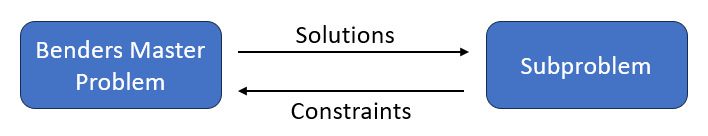
\includegraphics[width = 0.6\textwidth]{./images/BD.png}
  \end{figure}

  To avoid solving IP directly, we consider the LP relaxation of Problem \eqref{BD_master2}.
\end{frame}

% \begin{frame}{Deterministic Formulation}
%   Substitute the first constraint with $\sum_{j= 1}^{N} x_{ij} \geq s_{i}, i \in \mathcal{M}$, we can obtain the problem with lower bound supply. 
% \end{frame}

\begin{frame}{Deterministic Formulation}  %开始一张幻灯片
  To obtain an integral seat planning, we consider the following two deterministic formulations.
  \begin{columns}[c]  %开始进入分栏环境,居中设置
  \column{5cm}  %第一栏(左栏)宽度为5cm
  \scriptsize
  \begin{equation}\label{deter_upper}
    \begin{aligned}
    \max \quad & \sum_{i=1}^{M}  \sum_{j= 1}^{N} (n_i- s) x_{ij} \\
    \text {s.t.} \quad & \sum_{j= 1}^{N} x_{ij} {\color{red} \leq} s_{i}^{0}, \quad i \in \mathcal{M}, \\
    & \sum_{i=1}^{M} n_{i} x_{ij} \leq L_j, j \in \mathcal{N} \\
    & x_{ij} \in \mathbb{Z}_{+}, \quad i \in \mathcal{M}, j \in \mathcal{N}.
    \end{aligned}
  \end{equation}
  \column{5cm}
  \scriptsize
  \begin{equation}\label{deter_lower}
    \begin{aligned}
    \max \quad & \sum_{i=1}^{M}  \sum_{j= 1}^{N} (n_i- s) x_{ij} \\
    \text {s.t.} \quad & \sum_{j= 1}^{N} x_{ij} {\color{red} \geq} s_{i}^{1}, \quad i \in \mathcal{M}, \\
    & \sum_{i=1}^{M} n_{i} x_{ij} \leq L_j, j \in \mathcal{N} \\
    & x_{ij} \in \mathbb{Z}_{+}, \quad i \in \mathcal{M}, j \in \mathcal{N}.
    \end{aligned}
  \end{equation}
  \end{columns}  %分栏环境结束
  Problem \eqref{deter_upper} can generate a feasible seat planning.

  Problem \eqref{deter_lower} can generate a seat planning no inferior than any given feasible seat planning.
\end{frame}


\begin{frame}{Obtain The Feasible Seat Planning}
      \begin{description}
        \item[Step 1.] Obtain the solution, $\mathbf{x}^{*}$, by benders decomposition. Aggregate $\mathbf{x}^{*}$ to the number of each group type, ${s}_{i}^{0} =\sum_{j} x^{*}_{ij}, i \in \mathbf{M}$.

        \item[Step 2.] Solve problem \eqref{deter_upper} to obtain the optimal solution, $\mathbf{x}^{1}$. Aggregate $\mathbf{x}^{1}$ to the number of each group type, ${s}_{i}^{1} = \sum_{j} x^{1}_{ij}, i \in \mathbf{M}$.
        
        \item[Step 3.] Solve problem \eqref{deter_lower} to obtain the optimal solution, $\mathbf{x}^{2}$. Aggregate $\mathbf{x}^{2}$ to the number of each group type, ${s}_{i}^{2} = \sum_{j} x^{2}_{ij}, i \in \mathbf{M}$.
    
        \item[Step 4.] For each row, construct a full pattern.
     \end{description}
\end{frame}
    % !TeX root = ../main.tex

\section{Seat Planning with Deterministic Demand}
    \frame{\sectionpage}

  \begin{frame}{Deterministic Formulation}  %开始一张幻灯片
    Seat planning problem with given demand $\bm{d}$:

    \begin{equation}\label{deter_upper}
      \begin{aligned}
      \max \quad & \sum_{i=1}^{M}  \sum_{j= 1}^{N} (n_i- \delta) x_{ij} \\
      \text {s.t.} \quad & \sum_{j= 1}^{N} x_{ij} \leq d_{i}, \quad i \in \mathcal{M}, \\
      & \sum_{i=1}^{M} n_{i} x_{ij} \leq L_j, j \in \mathcal{N}, \\
      & x_{ij} \in \mathbb{Z}_{+}, \quad i \in \mathcal{M}, j \in \mathcal{N}.
      \end{aligned}
    \end{equation}
    Objective: maximize the number of people accommodated.

    $x_{ij}$: the number of group type $i$ in row $j$.
  \end{frame}

  \begin{frame}{Property}
    In the LP relaxation of problem \eqref{deter_upper}, there exists an index $v$ such that the optimal solutions satisfy the following conditions:

    \begin{itemize}
      \item For $i = 1,\ldots, v-1$ and for all $j$, $x_{ij}^{*} = 0$. 
      % indicating that no group type $i$ are assigned to any rows before index $v$.
      \item For $i = v+1,\ldots, M$, $\sum_{j} x_{ij}^{*} = d_{i}$. 

      \item For $i = v$, $\sum_{j} x_{ij}^{*} = \frac{L - \sum_{i = v+1}^{M} {d_i n_i}}{n_v}$ 
      % This quantity is determined by the available supply, which is calculated as the remaining seats after accommodating the demands for group types $v+1$ to $M$, divided by the size of group type $v$, denoted as $n_v$.
    \end{itemize}

    When the demand is way smaller than the number of seats, the seat planning obtained from problem \eqref{deter_upper} does not utilize all seats. We aim to generate a seat planning utilizing all seats while ensuring that the demand requirements are met.
  \end{frame}

  \begin{frame}{Generate The Full or Largest Pattern}
    Specifically, we can convert a given specific pattern into a largest or full pattern while ensuring that the original group type requirements are met. Our objective is to generate the pattern with maximal people.

    Mathematically, for any pattern $\bm{h} = (h_1, \ldots, h_M)$, we seek to find a pattern $\bm{h}{'} = (h_1{'}, \ldots, h_M{'})$ that satisfies the following programming.

    \begin{equation*}\label{full_largest}
      \begin{aligned}
      \max \quad & |\bm{h}{'}| \\
      \text {s.t.} \quad & h_1{'} \geq h_1 \\
      &  h_1{'} + h_2{'} \geq h_1 + h_2 \\
      & \cdots \\
      & h_1{'} + \ldots + h_M{'} \geq h_1 + \ldots + h_M.
      \end{aligned}
    \end{equation*}
  \end{frame}

  \begin{frame}{Algorithm to Generate The Full or Largest Pattern}
    For each row $j$, let $\beta_{j} = L_{j} - \sum_{i} n_{i} x_{ij}$. We aim to allocate the remaining unoccupied seats($\beta_{j}$) in row $j$ in a way that maximizes the number of planned groups that become the largest in size.
    \vspace{0.5cm}
    
    Allocation scheme of $\beta_{j}$:
    \vspace{0.5cm}

    \begin{scriptsize}
      Let $k = \min\{i | h_i > 0\}$ for a pattern $\bm{h}$.

      \begin{itemize}
        \item If $k \neq M$, $h_{k} \gets h_{k} -1$, $h_{\min_{\{(k+\beta_{j}), M\}}} \gets h_{\min_{\{(k+\beta_{j}), M\}}} +1$, $\beta_{j} \gets \beta_{j} - \max\{1, M - k\}$. Continue this procedure until the pattern is largest or $\beta_{j} =0$.
        \item If $k = M$ and $\beta_{j} > 0$, continue the following procedure until $\beta < n_{1}$.
        \item[-] When $\beta \geq n_{M}$, $q \gets \lfloor\frac{\beta}{n_M}\rfloor$, $\beta_{j} \gets \beta_{j} - q n_M$, $h_{M} \gets h_{M} + q$.
        \item[-] When $n_{1} \leq \beta_{j} < n_{M}$, $h_{\beta_{j}-n_1+1} \gets h_{\beta_{j}-n_1+1} + 1$, $\beta_{j} \gets 0$.
        % \item[] assign $\beta$ in a greedy way.
      \end{itemize}  
    \end{scriptsize}
    
  \end{frame}
    %You can put the frames directly into the presentation, but using the input command and writing them in separate .tex files might be more organized

    \section{}
    \begin{frame}{}
        \centering
            \Huge\bfseries
        \textcolor{orange}{The End}
    \end{frame}
\end{document}
